%!TEX root = ../dissertation.tex
\chapter{Other co-authored publications}
\label{app:other-publications}

\ifdraft{%
	\section{Astrin et al. (2016): Towards a DNA barcode reference database for spiders and harvestmen of germany}
	\emptypages{24} % Astrin 2016
	\section{Kraaijeveld et al. (2016): Decay of sexual trait genes in an asexual parasitoid wasp}
	\emptypages{11} % Kraaijeveld2016
	\section{Struck et al. (2014): Platyzoan paraphyly based on phylogenomic data supports a noncoelomate ancestry of Spiralia}
	\emptypages{17} % Struck2014
	\section{Peters et al. (2014): The evolutionary history of holometabolous insects inferred from transcriptome-based phylogeny and comprehensive morphological data}
	\emptypages{16} % Peters2014
	\section{Misof et al. (2014): Phylogenomics resolves the timing and pattern of insect evolution}
	\emptypages{5} % Misof2014
	\section{DellAmpio et al. (2014): Decisive data sets in phylogenomics: lessons from studies on the phylogenetic relationships of primarily wingless insects}
	\emptypages{11} % Dell'Ampio 2014
	\section{Niehuis et al. (2012): Genomic and morphological evidence converge to resolve the enigma of Strepsiptera}
	\emptypages{5} % Niehuis2012
}%
{%
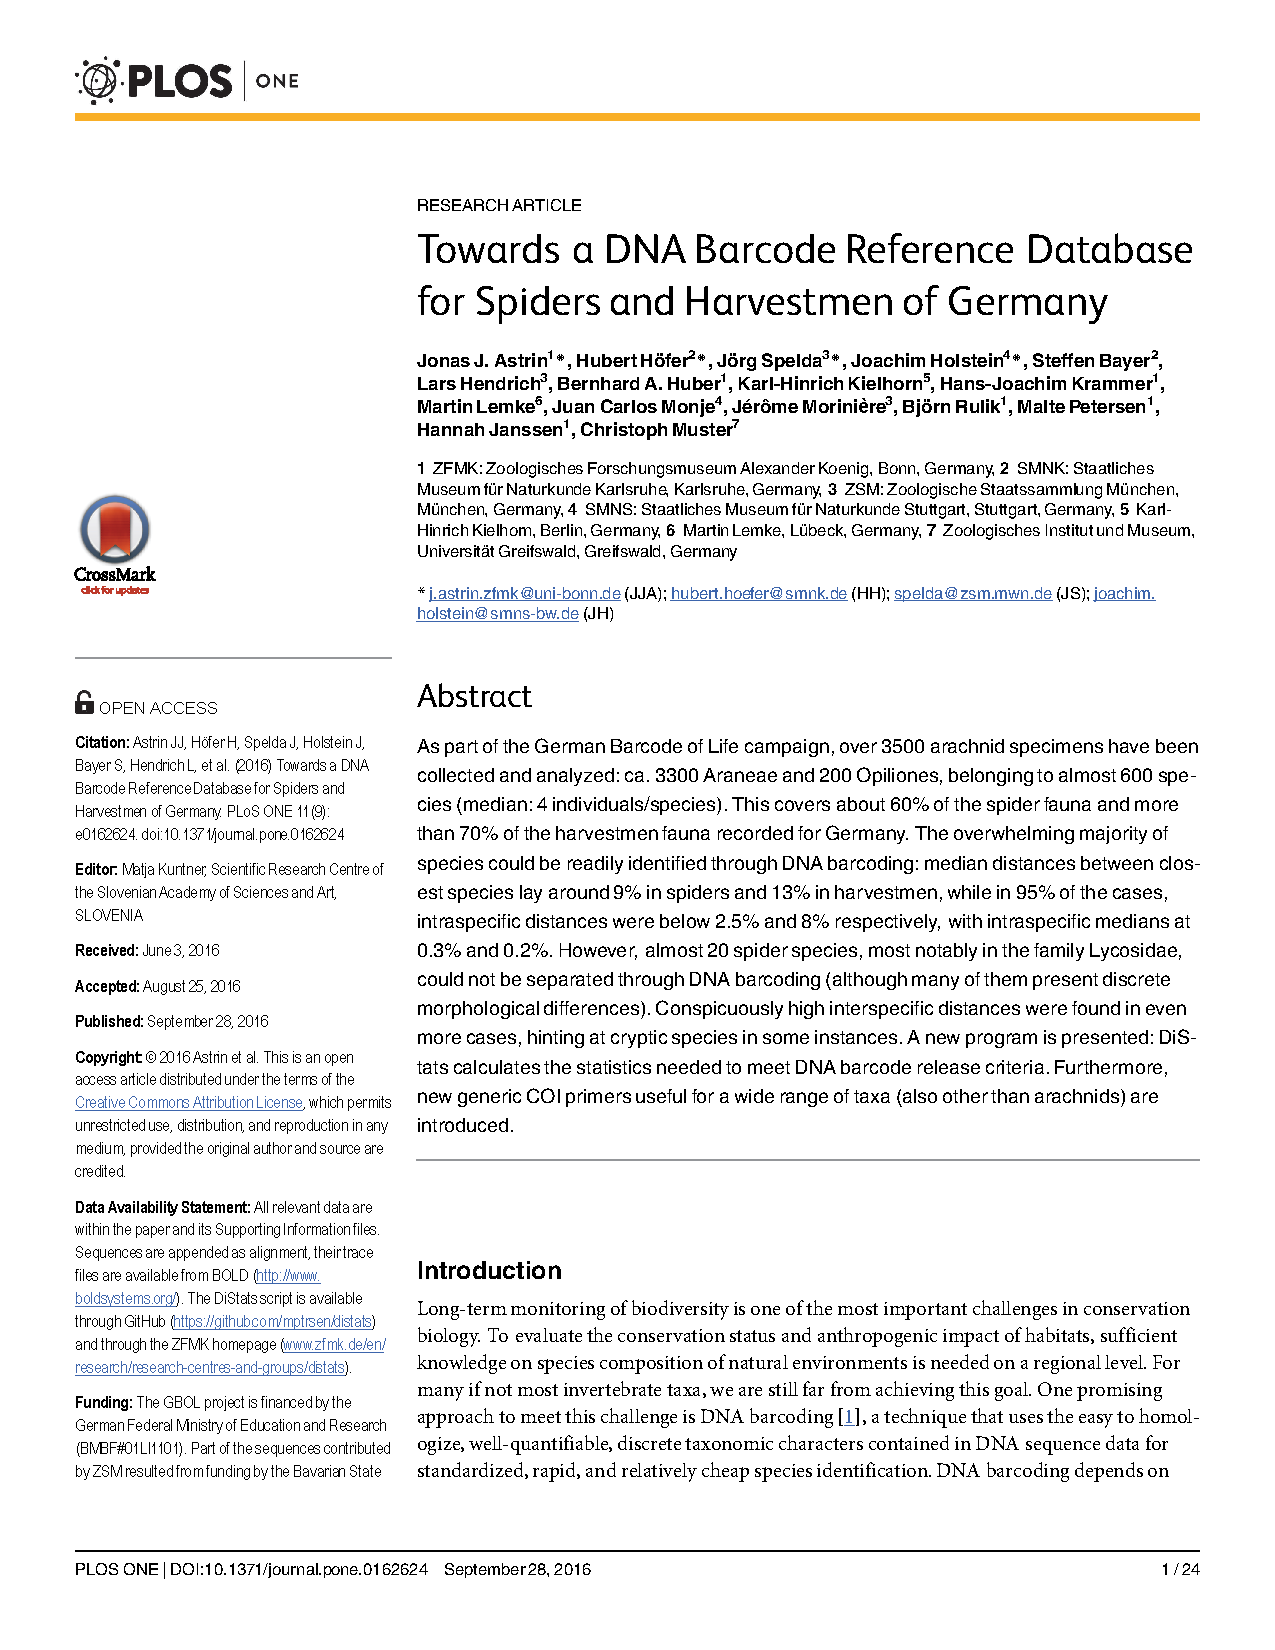
\includepdf[addtotoc={1,section,1,Astrin et al. (2016): Towards a DNA barcode reference database for spiders and harvestmen of germany,app:Astrin2016},pages=-]{appendix/B/Astrin2016} % range without endpoints: from first to last
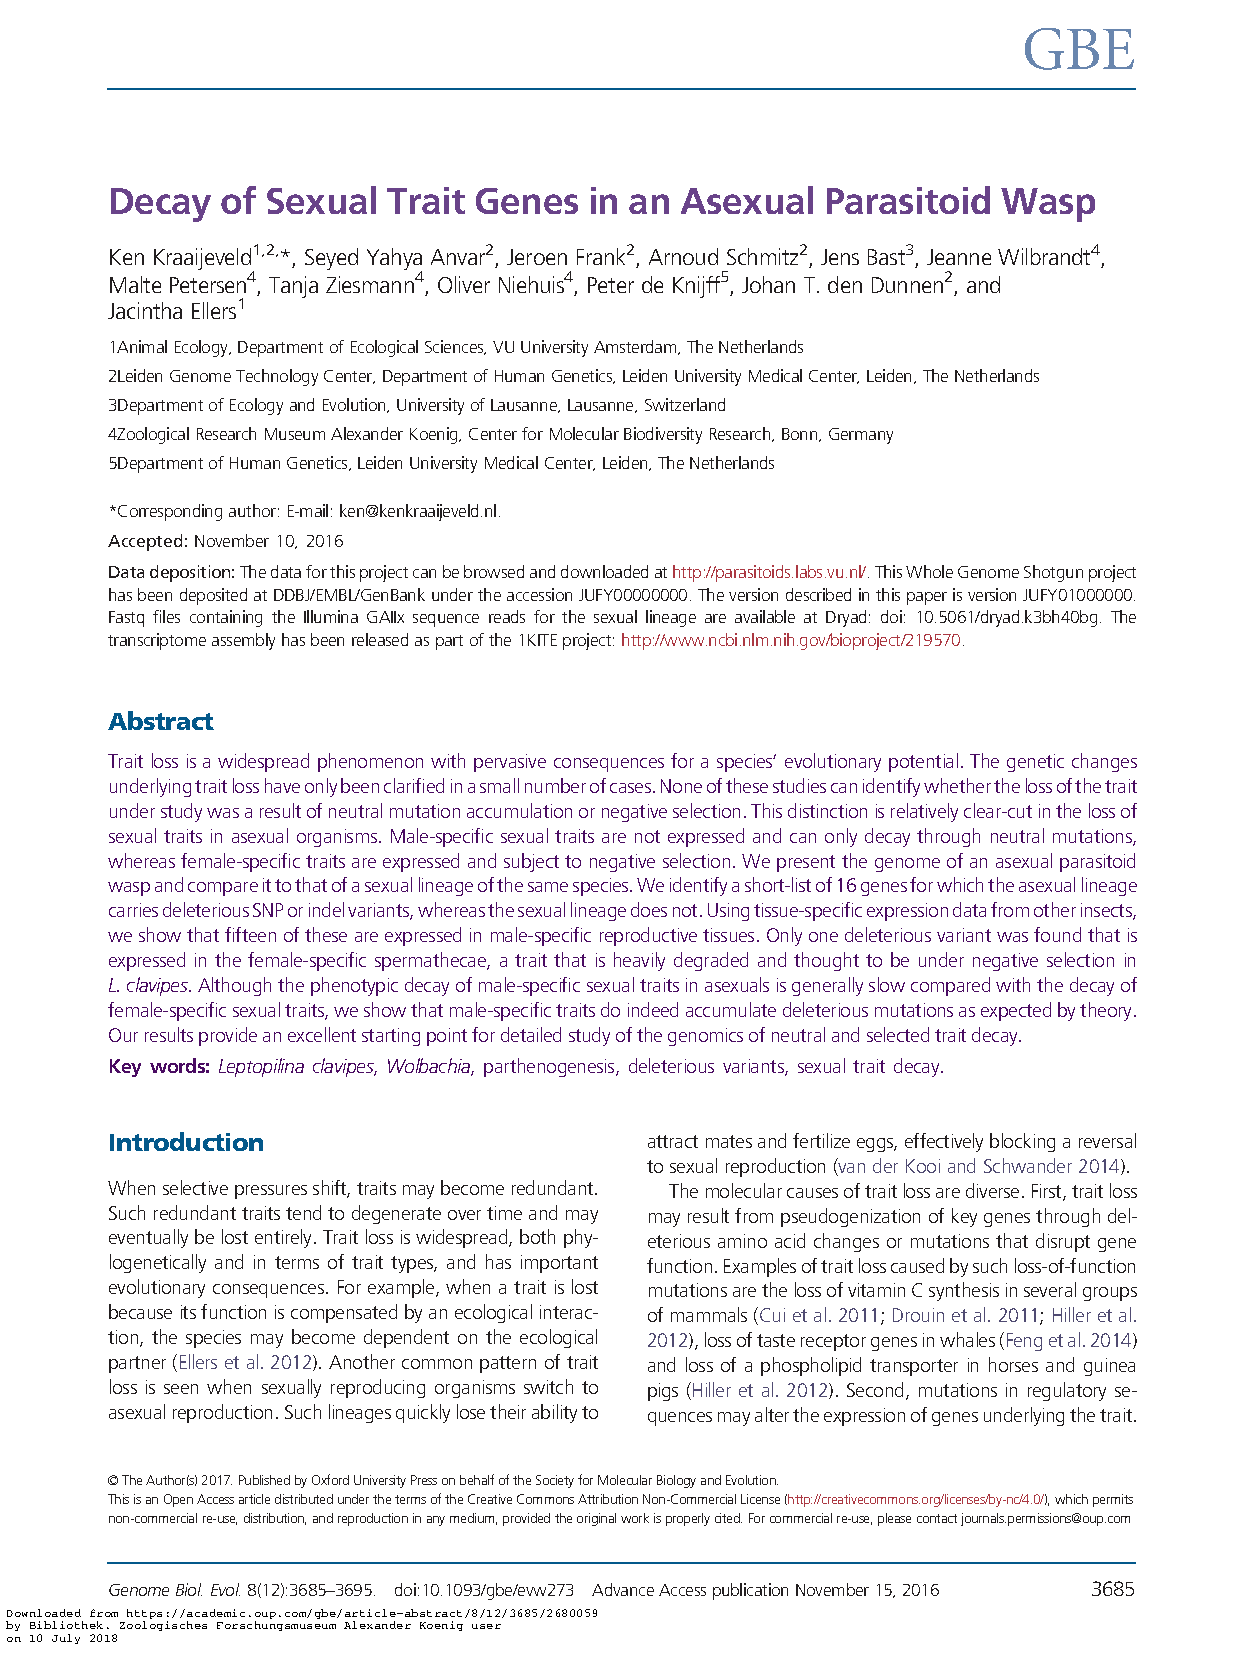
\includepdf[addtotoc={1,section,1,Kraaijeveld et al. (2016): Decay of sexual trait genes in an asexual parasitoid wasp,app:Kraaijeveld2016},pages=-]{appendix/B/Kraaijeveld2016} % range without endpoints: from first to last
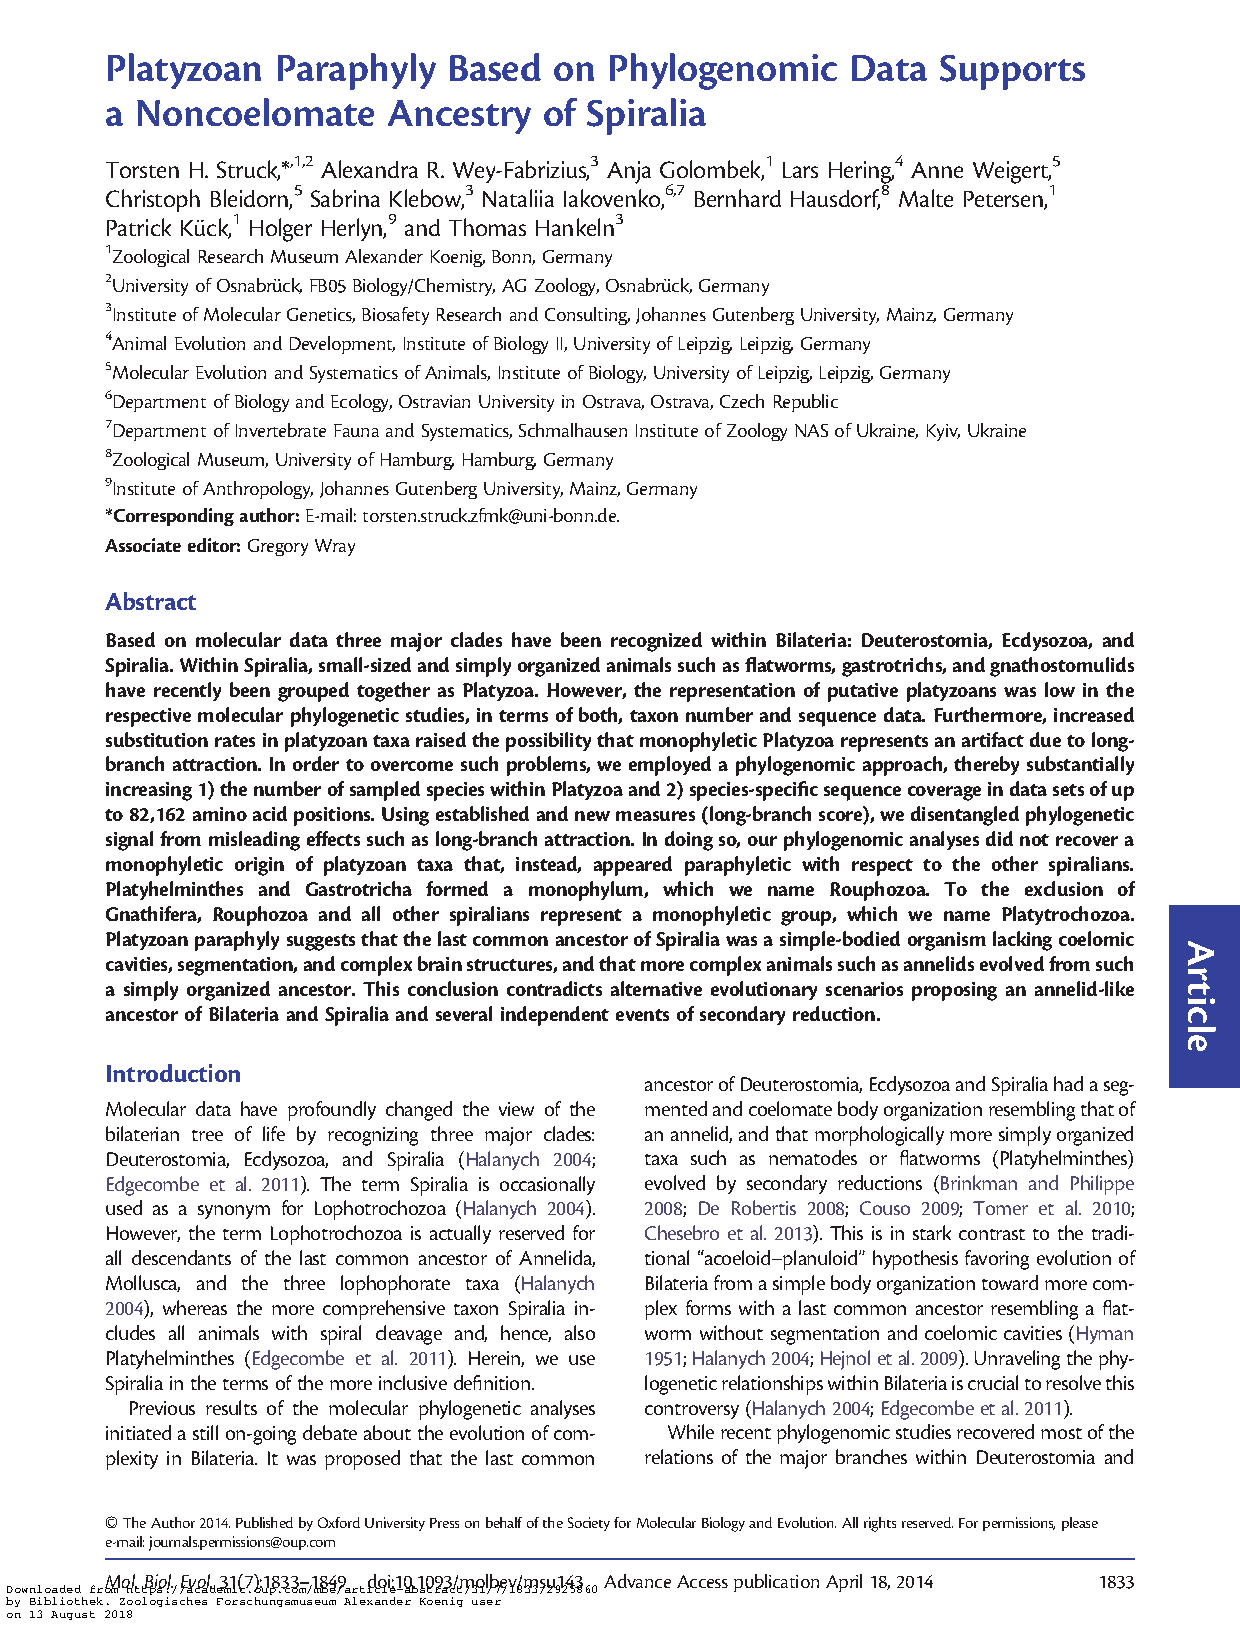
\includepdf[addtotoc={1,section,1,Struck et al. (2014): Platyzoan paraphyly based on phylogenomic data supports a noncoelomate ancestry of Spiralia,app:Struck2014},pages=-]{appendix/B/Struck2014} % range without endpoints: from first to last
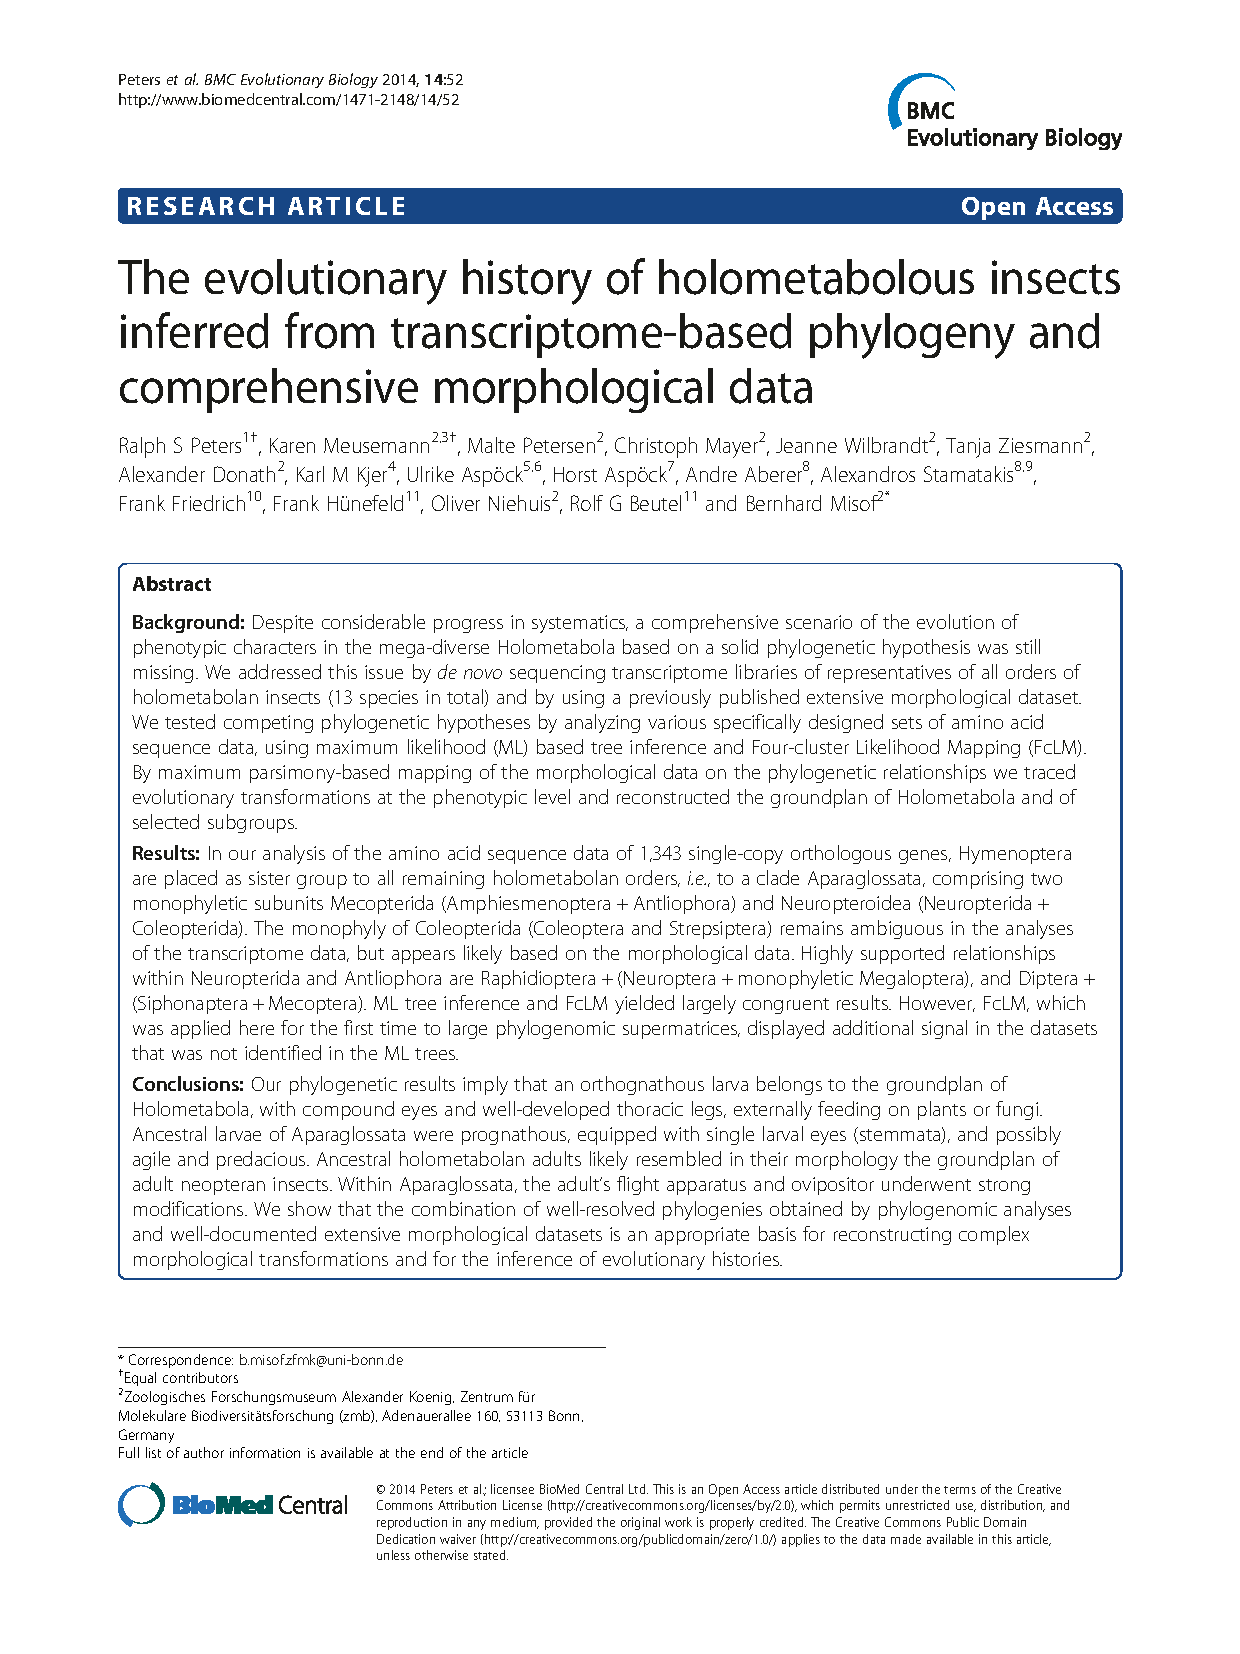
\includepdf[addtotoc={1,section,1,Peters et al. (2014): The evolutionary history of holometabolous insects inferred from transcriptome-based phylogeny and comprehensive morphological data,app:Peters2014},pages=-]{appendix/B/Peters2014} % range without endpoints: from first to last
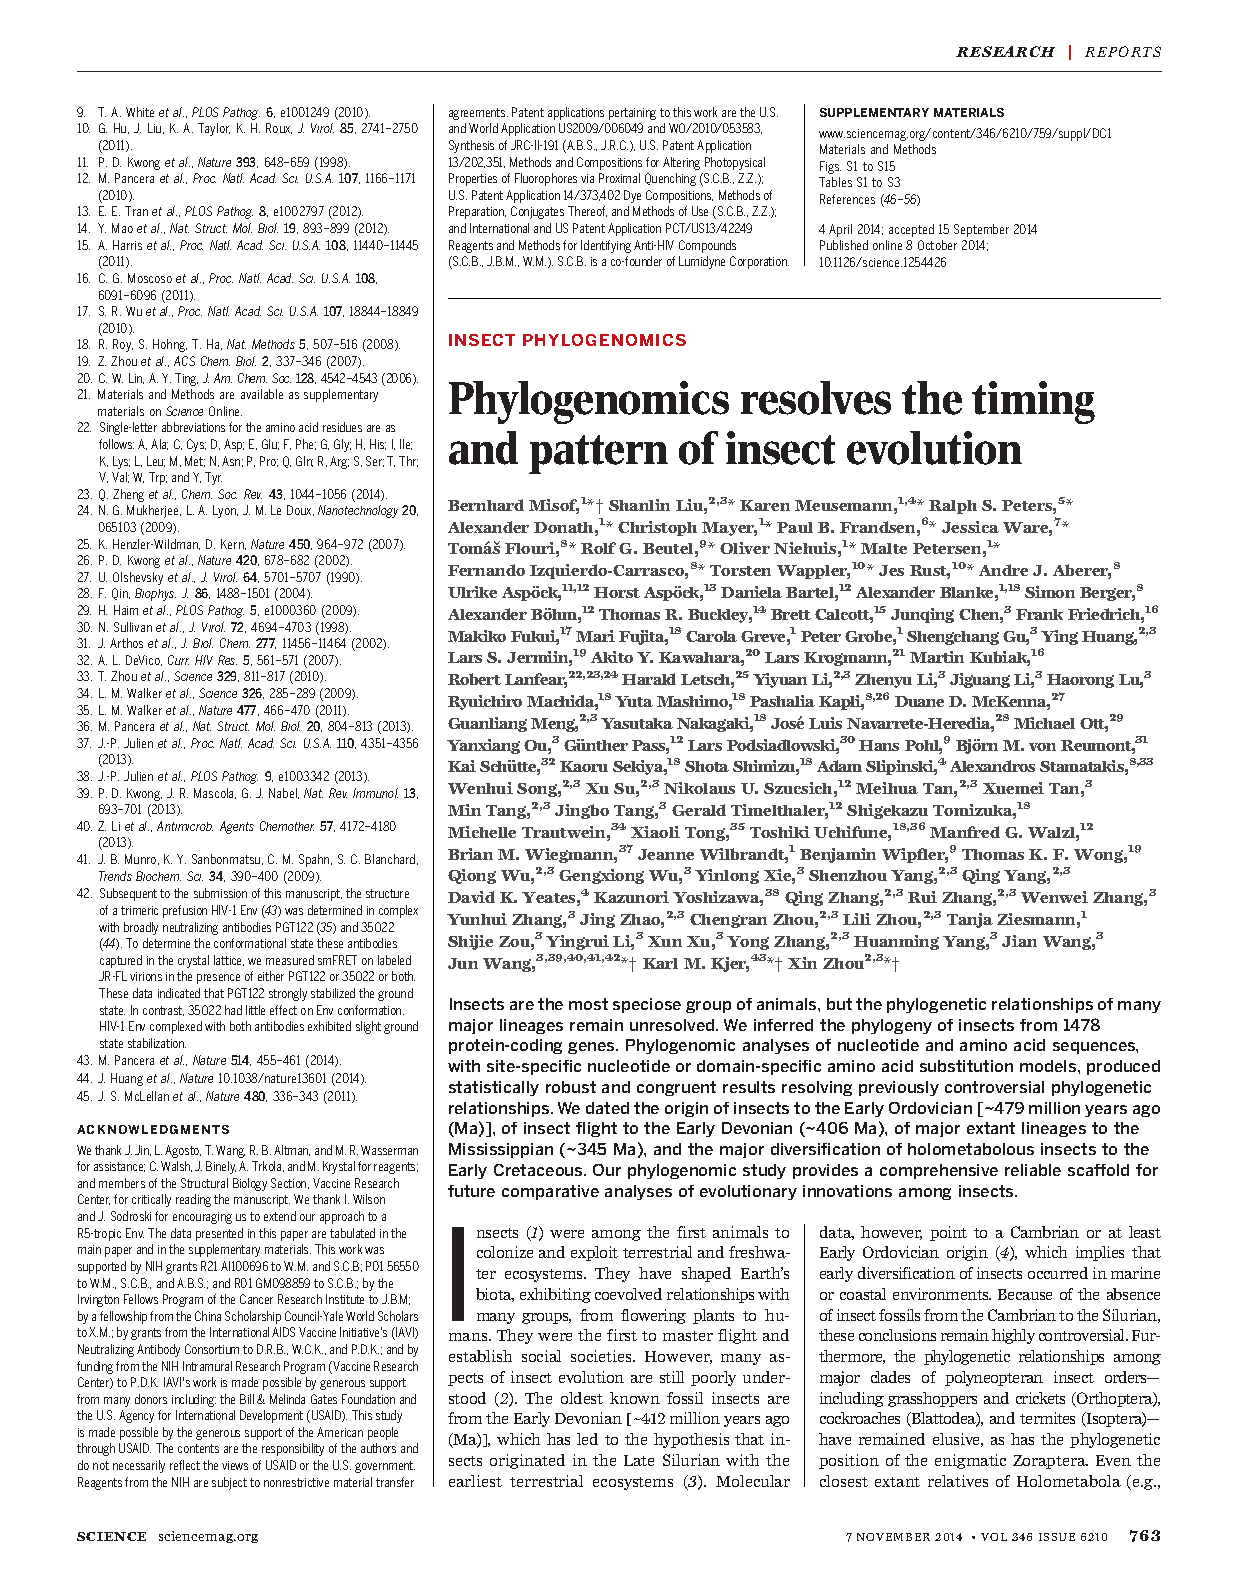
\includepdf[addtotoc={1,section,1,Misof et al. (2014): Phylogenomics resolves the timing and pattern of insect evolution,app:Misof2014},pages=-]{appendix/B/Misof2014} % range without endpoints: from first to last
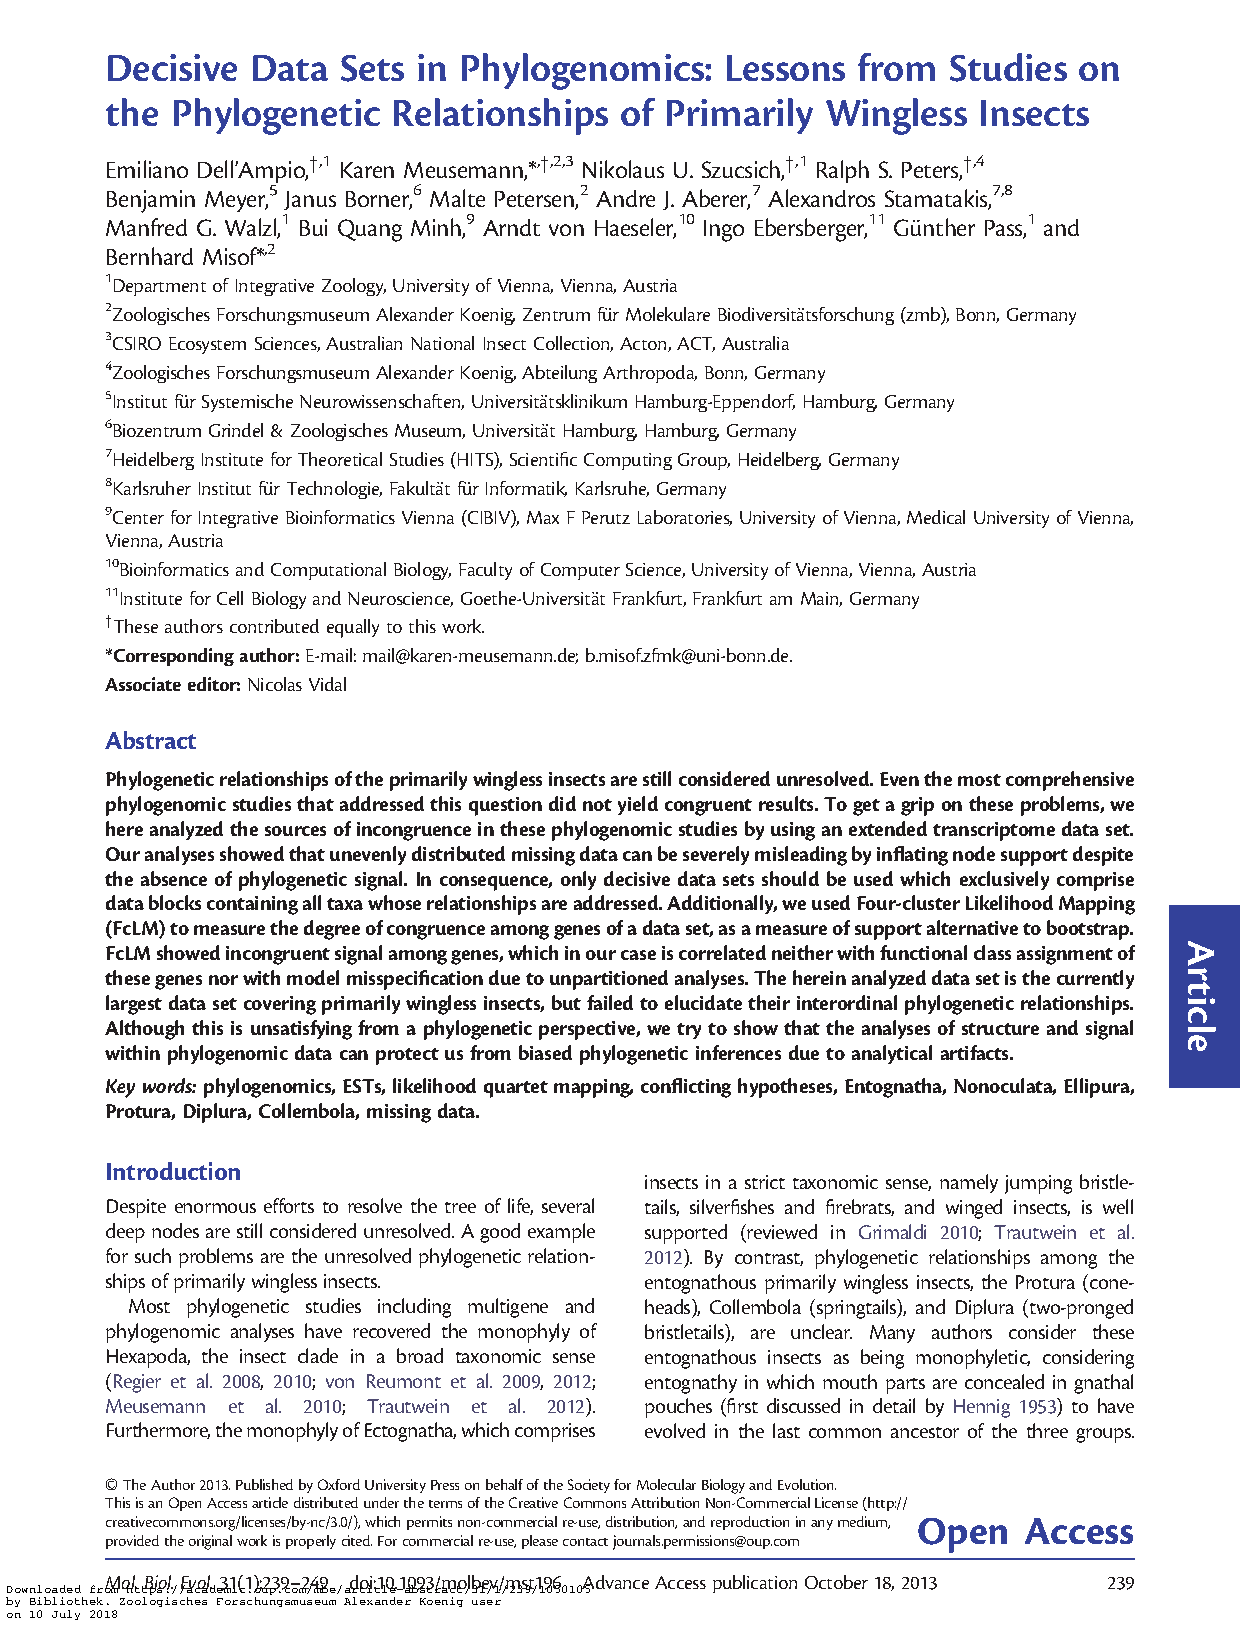
\includepdf[addtotoc={1,section,1,DellAmpio et al. (2014): Decisive data sets in phylogenomics: lessons from studies on the phylogenetic relationships of primarily wingless insects,app:DellAmpio2014},pages=-]{appendix/B/DellAmpio2014} % range without endpoints: from first to last
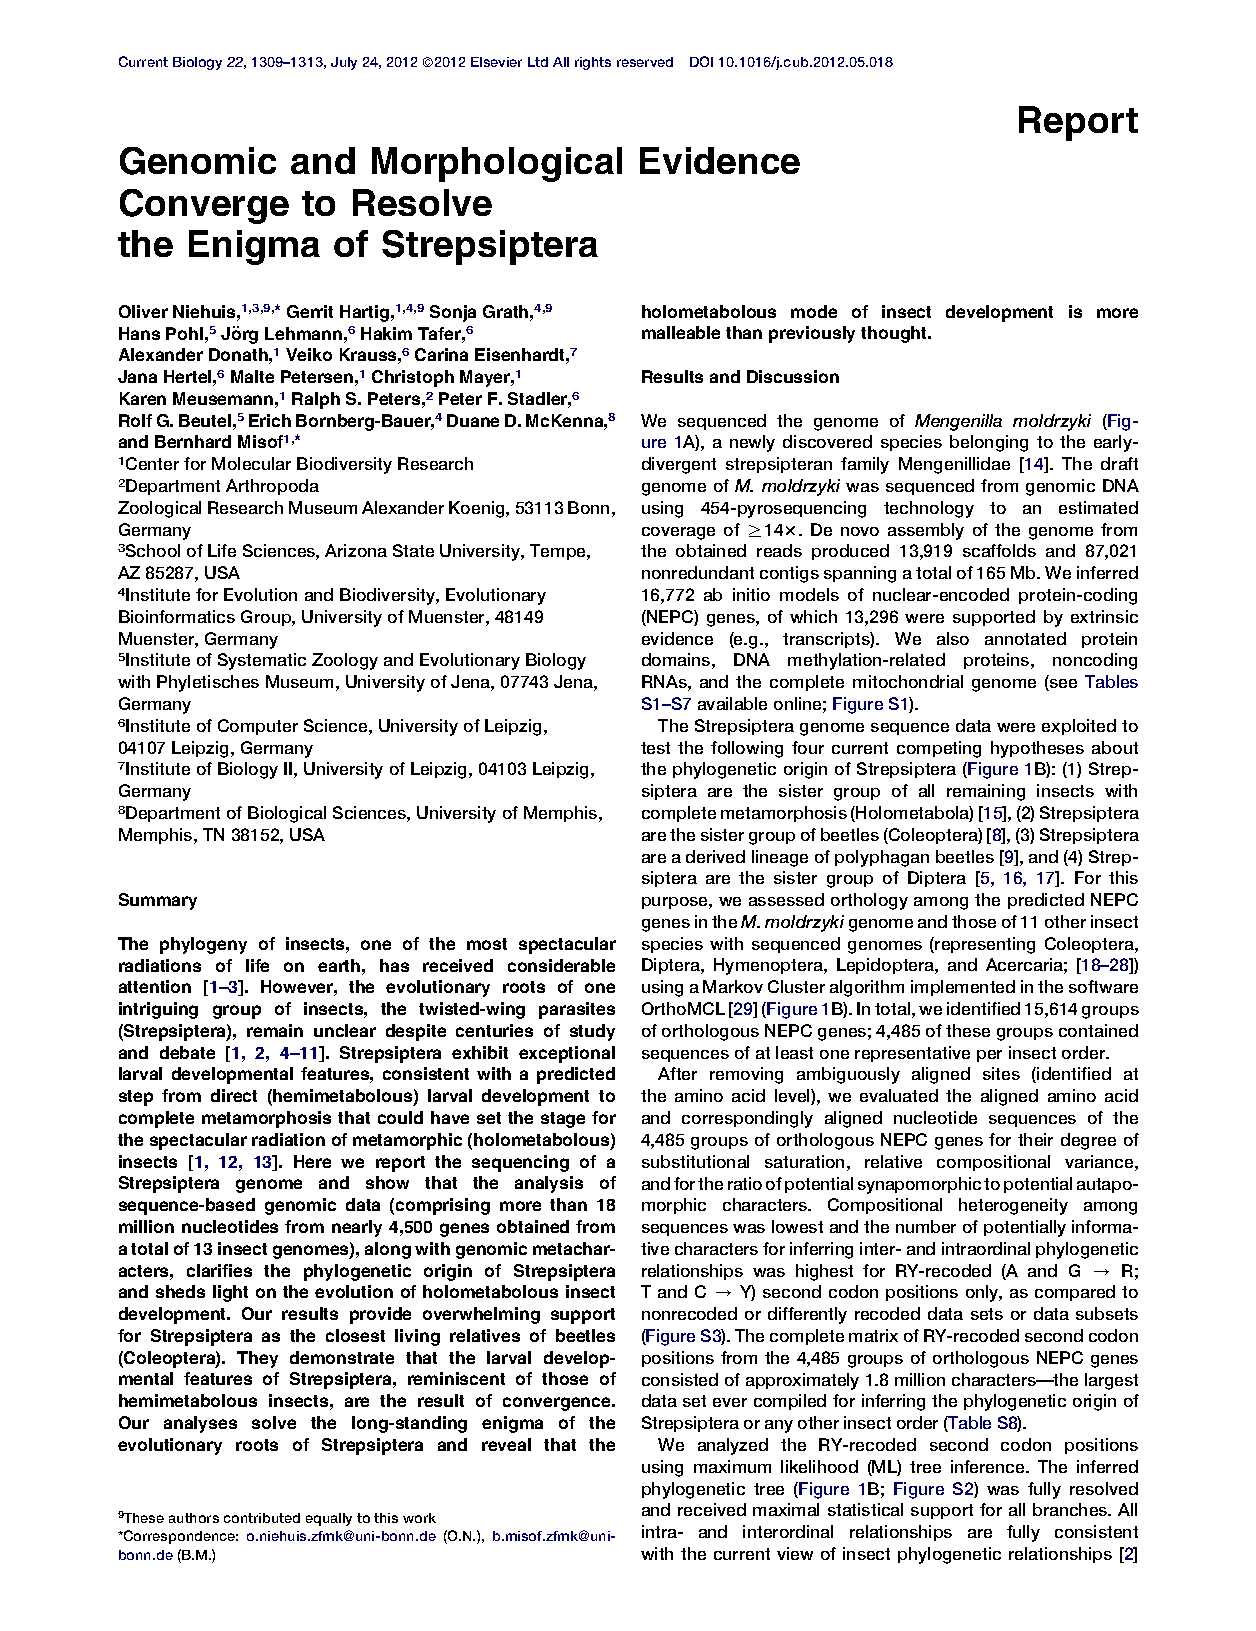
\includepdf[addtotoc={1,section,1,Niehuis et al. (2012): Genomic and morphological evidence converge to resolve the enigma of Strepsiptera,app:Niehuis2012},pages=-]{appendix/B/Niehuis2012} % range without endpoints: from first to last
}%
